\chapter{Relationships between words}
\label{sec:lexical}

\lettrine[lines=5,loversize=0.25]{T}{his} chapter describes experiments to discover optimal parameters for lexical similarity, and the behavioural patterns of the parameters.\footnotemark{}
\footnotetext{Much of the work in this chapter has appeared as \newcite{milajevs-sadrzadeh-purver:2016:ACL-SRW} at the ACL Student Workshop 2016.} Simlex-999 \cite{hill2014simlex} and MEN \cite{Bruni:2014:MDS:2655713.2655714} are the two datasets that are used for evaluation. They provide averaged values of similarity judgements between pairs of words.

The experiment results and selected parameters are reported on the datasets individually. Then, the model selection is performed on a combination of the two datasets. The results are selected using three methods: Max selection, where the best score is selected, cross-validation, which separates model selection and score computation, and a selection based on heuristics, here parameters are chosen by their influence.

The experiments show that while the best parameter selection depends on the dataset, there is a global optimal parameter selection that is good on all datasets. In general, we find that non-constant frequency component, context distribution smoothing and shifting should be used for high-dimensional spaces to compensate for the noise that is introduced by a large number of context features.

\section{Experiments on SimLex-999 dataset}
\label{sec:simlex-999}

SimLex-999 is a dataset to evaluate lexical semantic models \cite{hill2014simlex}. It tests how well a model captures similarity between word pairs. The dataset implicitly distinguishes similarity and relatedness, so related pairs such that \textit{coffee}, \textit{cup} are not considered to be similar in this dataset. It consists of 666 noun-noun pairs, 222 verb-verb pairs and 111 adjective-adjective pairs. The models are evaluated by computing the Spearman's-$\rho$ (the correlation of ranked model predictions with ranked human judgements). Minimum required difference for significance (MRDS, \citet{rastogi-vandurme-arora:2015:NAACL-HLT}) is used for statistical significance testing. For SimLex-999, $\sigma^{0.9}_{0.05} = 0.023$.\footnotemark{}
\footnotetext{The results are available at \url{\BASEURL/results_all.csv}.}

\subsection{Max selection}
\label{sec:max-selection-simlex}

\begin{wrapfigure}[7]{O}{0.5\textwidth}
  \vspace{-30pt}
  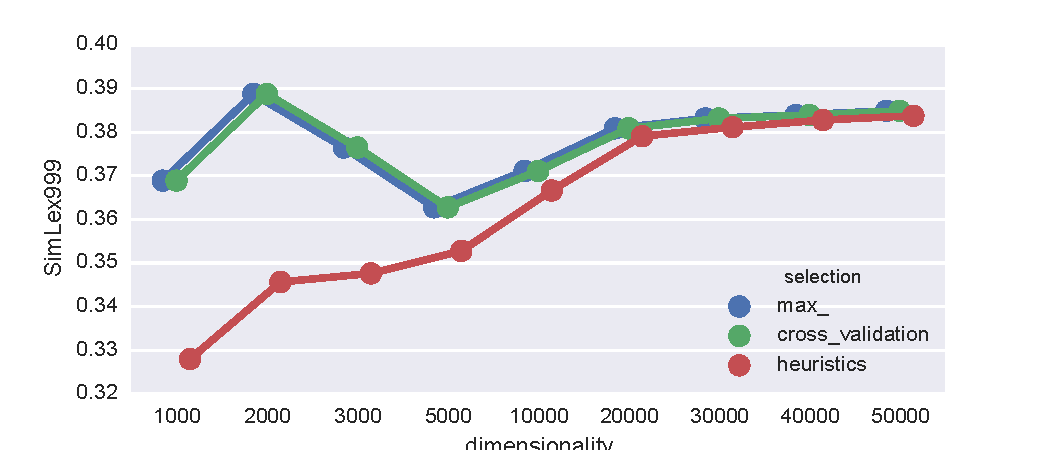
\includegraphics[width=0.5\textwidth]{supplement/figures/SimLex999-results}
  \caption{SimLex-999 results.}
  \label{fig:SimLex999-results}
\end{wrapfigure}

%%% Local Variables:
%%% mode: latex
%%% TeX-master: "../thesis"
%%% End:


Figure~\ref{fig:SimLex999-results} illustrates the results based on the best model selection and Table~\ref{tab:Simlex999-max-selection} shows the results together with chosen parameters. Note that maximum selection is identical with cross-validation: they pick the same models.

In general, model performance increases as dimensionality increases. There is no statistically significant difference between the scores with an exception of the 5\,000 model, which underperforms. The best result of 0.389 is achieved with a 2\,000 dimensional space. Model performance becomes stable for dimensions greater than 20\,000, which suggests that rare context features contribute very little to similarity estimation.

\begin{table}
  \centering

  \begin{tabular}{rrlllrl}
\toprule
 dimensionality &  SimLex999 &  freq &  discr &     cds &  neg &     similarity \\
\midrule
           1\,000 &      0.369 &     1 &   spmi &       1 &  0.2 &  inner\_product \\
           2\,000 &      0.389 &     1 &  scpmi &  global &  0.7 &  inner\_product \\
           3\,000 &      0.376 &     1 &   spmi &    0.75 &  0.2 &  inner\_product \\
           5\,000 &      0.363 &  logn &  scpmi &  global &  1.0 &            cos \\
          10\,000 &      0.371 &  logn &  scpmi &       1 &  0.7 &            cos \\
          20\,000 &      0.381 &  logn &  scpmi &    0.75 &  0.7 &            cos \\
          30\,000 &      0.383 &  logn &  scpmi &    0.75 &  0.7 &            cos \\
          40\,000 &      0.384 &  logn &  scpmi &    0.75 &  0.7 &            cos \\
          50\,000 &      0.385 &  logn &  scpmi &    0.75 &  0.7 &            cos \\
\bottomrule
\end{tabular}


  \caption{SimLex-999 Max selection.}
  \label{tab:Simlex999-max-selection}
\end{table}


As we see later in Section~\ref{sec:simlex-men} the best result is an example of overfitting. The 2\,000 dimensional model performs very well on SimLex-999 achieving the score of 0.389, but underperforms on MEN achieving the score of 0.660, while the model chosen using heuristics yields the score of 0.724 on MEN (the difference is statistically significant). In addition, the model selected by using heuristics is not statistically significantly different from the maximum result for this dimensionality (0.728, Figure~\ref{fig:SimLex999-transfer}).

For spaces with dimensionality less than 5\,000, the frequency parameter set to 1 and the inner product as the similarity measure yield the best results. Otherwise, cosine with \logNSCPMI/, smoothing $\alpha=0.75$ and shifting $k=0.7$ gives the best results. This supports our hypotheses that high-dimensional spaces benefit from a non-constant frequency (H\ref{hyp:freq}), smoothing of context distribution (H\ref{hyp:cds}) and the sparsity of vectors (H\ref{hyp:neg}).

\subsection{Heuristics}
\label{sec:heuristics-simlex}

% \begin{figure}

  \centering

  \begin{subfigure}[t]{0.49\textwidth}
    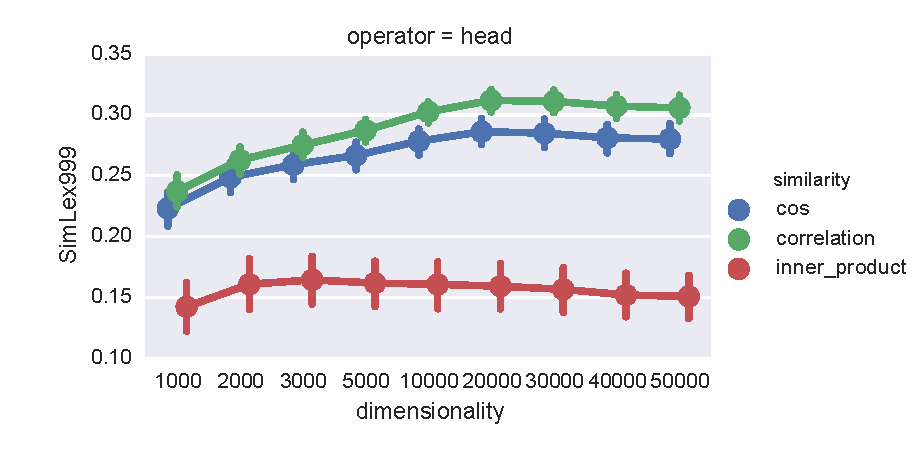
\includegraphics[width=\textwidth]{supplement/figures/SimLex999-interaction-similarity}
    \caption{similarity}
    \label{fig:SimLex999-interaction-similarity}
  \end{subfigure}
  \begin{subfigure}[t]{0.49\textwidth}
    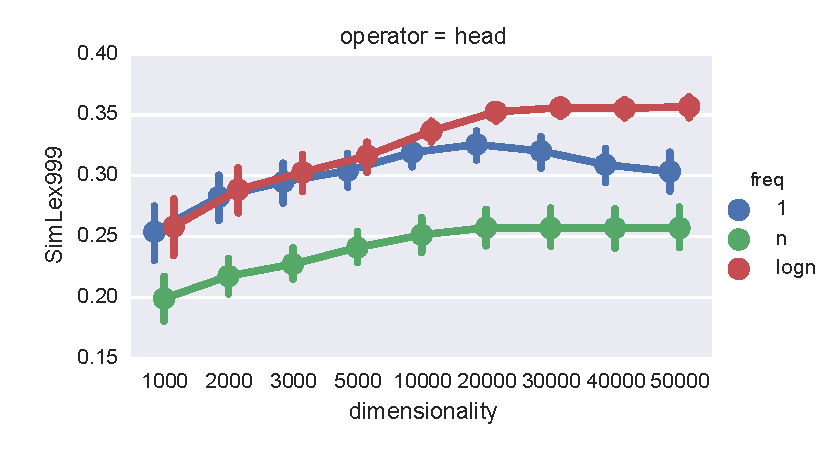
\includegraphics[width=\textwidth]{supplement/figures/SimLex999-interaction-freq}
    \caption{\texttt{freq}}
    \label{fig:SimLex999-interaction-freq}
  \end{subfigure}

  \begin{subfigure}[t]{0.49\textwidth}
    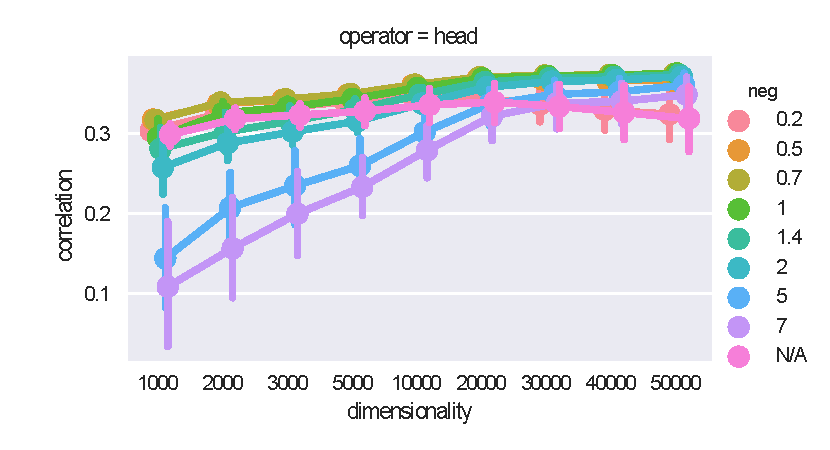
\includegraphics[width=\textwidth]{supplement/figures/SimLex999-interaction-neg}
    \caption{\texttt{neg}}
    \label{fig:SimLex999-interaction-neg}
  \end{subfigure}
  \begin{subfigure}[t]{0.49\textwidth}
    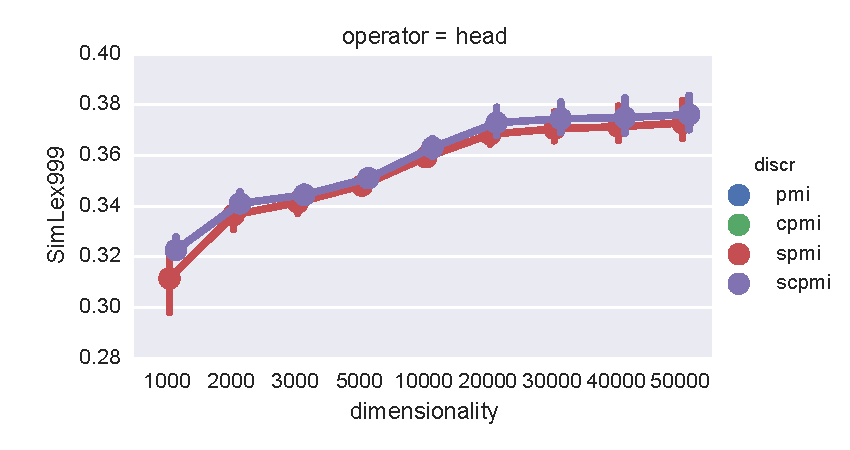
\includegraphics[width=\textwidth]{supplement/figures/SimLex999-interaction-discr}
    \caption{\texttt{discr}}
    \label{fig:SimLex999-interaction-discr}
  \end{subfigure}

  \begin{subfigure}[t]{0.49\textwidth}
    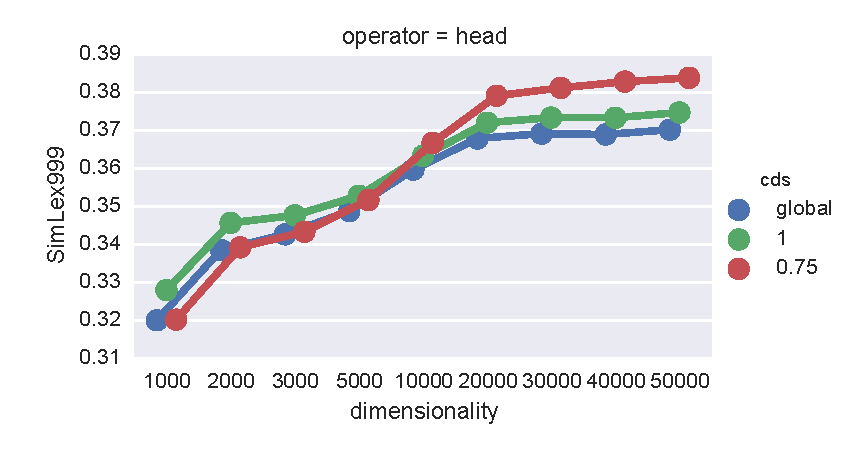
\includegraphics[width=\textwidth]{supplement/figures/SimLex999-interaction-cds}
    \caption{\texttt{cds}}
    \label{fig:SimLex999-interaction-cds}
  \end{subfigure}

  \caption{SimLex-999 parameter interaction. Parameters are shown in the order of their influence.}
  \label{fig:SimLex999-interaction}
\end{figure}

%%% Local Variables:
%%% mode: latex
%%% TeX-master: "../thesis"
%%% End:


Analysis of variance is used to obtain parameter influence. First, we fit a linear regression model that takes into account all model parameters. The similarity score is a dependent variable, while the parameters of a similarity model are independent variables. In addition to individual parameter influence, we also consider their two-way interactions. The full linear model is defined as:
\begin{equation}
  \text{\it score} \sim \sum_{p \in P}p + \sum_{p, p' \in P \times P}p \cdot p'
\end{equation}
where $P$ is the set of parameters, in our case $P = \{\text{\it freq}, \text{\it discr}, \text{\it cds}, \text{\it neg}, \text{\it similarity} \}$.

The linear model achieves an adjusted $R^2$ value of 0.867, indicating that the linear model is able to predict the performance of a similarity model based on the parameters $P$ quite well.

After fitting a model on the full set of parameters,  we fit six ``restricted'' linear models, each of them excluding a parameter $\bar p$:
\begin{equation}
  \text{\it score} \sim \sum_{p \in P \setminus \{\bar p\} }p + \sum_{p, p' \in (P \setminus \{\bar p\}) \times (P \setminus \{\bar p\})}p \cdot p'
\end{equation}

\begin{table}
  \centering

  \begin{tabular}{rrlllll}
\toprule
 dimensionality &  SimLex999 &  freq &  discr &   cds &  neg &   similarity \\
\midrule
           1\,000 &      0.328 &  logn &  scpmi &     1 &  0.7 &  correlation \\
           2\,000 &      0.346 &  logn &  scpmi &     1 &  0.7 &  correlation \\
           3\,000 &      0.348 &  logn &  scpmi &     1 &  0.7 &  correlation \\
           5\,000 &      0.353 &  logn &  scpmi &     1 &  0.7 &  correlation \\
          10\,000 &      0.367 &  logn &  scpmi &  0.75 &  0.7 &  correlation \\
          20\,000 &      0.379 &  logn &  scpmi &  0.75 &  0.7 &  correlation \\
          30\,000 &      0.381 &  logn &  scpmi &  0.75 &  0.7 &  correlation \\
          40\,000 &      0.383 &  logn &  scpmi &  0.75 &  0.7 &  correlation \\
          \textbf{50\,000} &      \textbf{0.384} &  \textbf{logn} &  \textbf{scpmi} &  \textbf{0.75} &  \textbf{0.7} &  \textbf{correlation} \\
\bottomrule
\end{tabular}


  \caption{SimLex-999 selection based on heuristics. The highest value is 0.384.
  The values that are grater than 0.361 are indistinguishable from the highest score.}
  \label{tab:Simlex999-heuristics-selection}
\end{table}


\begin{wraptable}[8]{O}{0.5\textwidth}
  \vspace{-1em}
  \centering

  \begin{tabular}{lr}
\toprule
      parameter &  partial $R^2$ \\
\midrule
     similarity &       0.38 \\
           freq &       0.27 \\
            neg &       0.24 \\
 dimensionality &       0.08 \\
          discr &       0.08 \\
            cds &       0.06 \\
\bottomrule
\end{tabular}


  \caption{SimLex-999 feature ablation}
  \label{tab:SimLex999-ablation}
\end{wraptable}


We compute $R^2$ scores of the models that exclude a parameter. The difference of the $R^2$ sore of the full model and the $R^2$ score of a restricted model is the partial $R^2$ score of the excluded parameter. Table~\ref{tab:SimLex999-ablation} shows partial $R^2$ scores for all the parameters. The most influential parameters, in decreasing order, are similarity, \texttt{freq} and \texttt{neg}, the contribution of other parameters to model performance estimation is minimal.

To identify whether one parameter choice outperforms another, the mean performance of both is estimated and the difference between them is compared. If the difference is less than the MRDS for the dataset, then the parameter choices are statistically indistinguishable.

% \begin{wrapfigure}{O}{0.5\textwidth}
\begin{figure}
  % \vspace{-30pt}
  \centering

  \begin{subfigure}[t]{0.49\textwidth}
    \hspace{-20pt}
  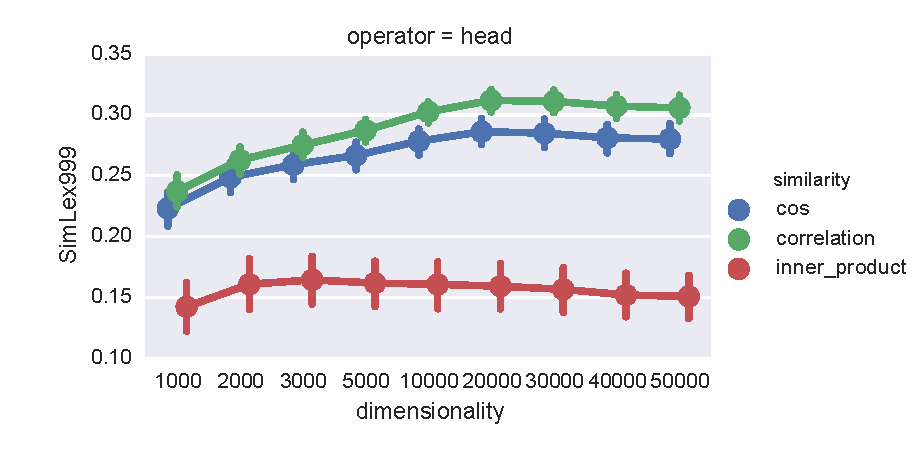
\includegraphics[width=1.1\textwidth]{supplement/figures/SimLex999-interaction-similarity}

  \caption{Similarity measure}
  \label{fig:SimLex999-similarity}

  \end{subfigure}
  \begin{subfigure}[t]{0.49\textwidth}

  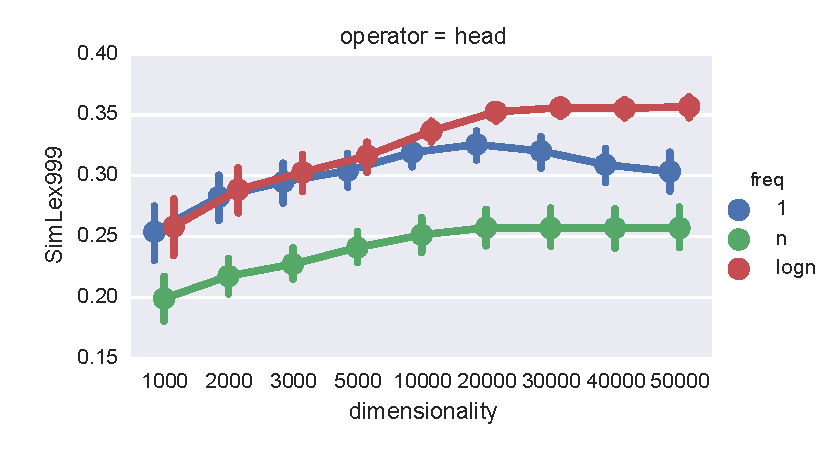
\includegraphics[width=\textwidth]{supplement/figures/SimLex999-interaction-freq}

  \caption{\texttt{freq}}
  \label{fig:SimLex999-freq}

  \end{subfigure}


  \begin{subfigure}[t]{0.49\textwidth}
  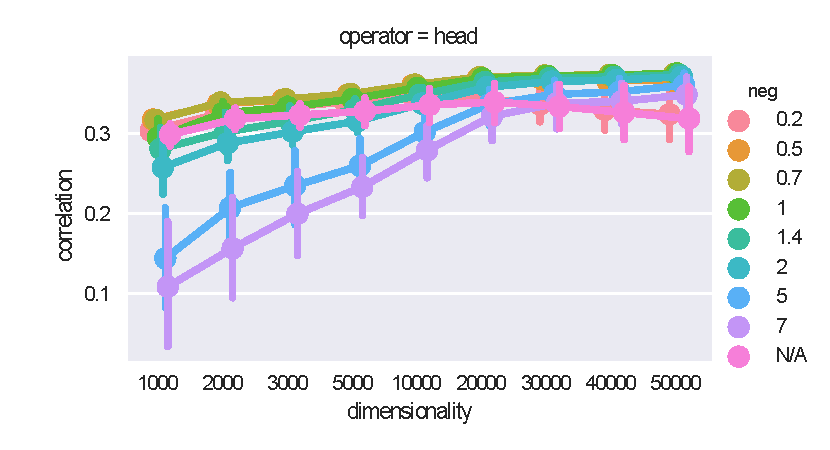
\includegraphics[width=\textwidth]{supplement/figures/SimLex999-interaction-neg}

  \caption{\texttt{neg}}
  \label{fig:SimLex999-neg}
  \end{subfigure}
  \begin{subfigure}[t]{0.49\textwidth}
  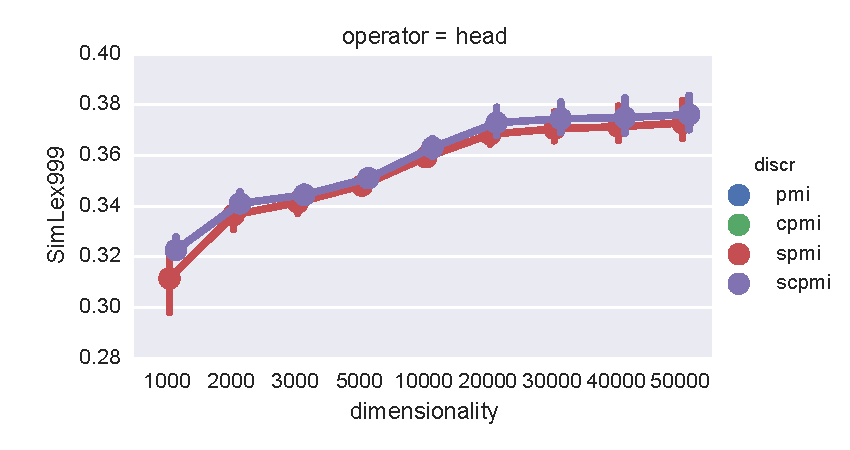
\includegraphics[width=\textwidth]{supplement/figures/SimLex999-interaction-discr}

  \caption{\texttt{discr}}
  \label{fig:SimLex999-discr}
  \end{subfigure}
  
  \caption[SimLex-999 influence of the similarity measure, \texttt{freq}, \texttt{neg} and \texttt{discr}]{SimLex-999 influence of the similarity measure, \texttt{freq}, \texttt{neg} and \texttt{discr}. Error bars indicate the 95\% confidence interval over the group of results.}
\end{figure}

Figure~\ref{fig:SimLex999-similarity} shows the average performance of similarity measures. Correlation outperforms all other measures for all dimensions and peaks at the dimensionality of 20\,000, as Table~\ref{tab:Simlex999-heuristics-selection} shows. However, for $D < 10\,000$, the difference between correlation-based and cosine-based similarity measures is not statistically significant, while it is for $D \ge 10\,000$. This supports H\ref{hyp:similarity} that correlation performs well with high-dimensional spaces.

The influence of \texttt{freq}, the second parameter, is shown in Figure~\ref{fig:SimLex999-freq}. $\log n$ frequency outperforms other choices for all dimensions. At 20\,000 and more dimensions, $\log n$ statistically significantly outperforms $1$. Also, $\log n$'s performance stabilises: variance decreases and the performance stays constant. Taking into account that for $D < 20\,000$ the difference between $1$ and $\log n$ is not statistically significant, H\ref{hyp:freq} is supported in this case as well, suggesting that for low-dimensional spaces the frequency component is unnecessary.

The third parameter \texttt{neg}, with a value of 0.7, shows the best performance (Figure~\ref{fig:SimLex999-neg}), but 0.5 and 1 are statistically indistinguishable from it. With more than 3\,000 dimensions, the difference between 0.7 and 1.4 is statistically insignificant. Similarly, 2 is not statistically different with more than 10\,000 dimensions and 5 with more than 30\,000 dimensions.

The performance of \texttt{neg} set to 7 increases as dimensionality increases, but the difference with 0.7 is statistically significant for all dimensions. We expect that with more dimensions, the difference between 0.7 and 7 becomes statistically insignificant.

Models with \texttt{neg} set to 0.2 become statistically different with more than 30\,000 dimensions.
 
The score variance is much lower for high-dimensional spaces than for low-dimensional spaces, so for high-dimensional more choice of \texttt{neg} are statistically indistinguishable from the best choice of 0.7 This gives support to H\ref{hyp:var} that high-dimensional models are more likely to outperform low-dimensional models.

Also, lower $k$ values, which make vectors denser, lead to higher performance in low-dimensional spaces, supporting H\ref{hyp:neg} that expects low-dimensional models benefit from dense vectors.

% \begin{figure}[h]
\begin{wrapfigure}[5]{O}{0.5\textwidth}
  \vspace{-30pt}
  \centering

  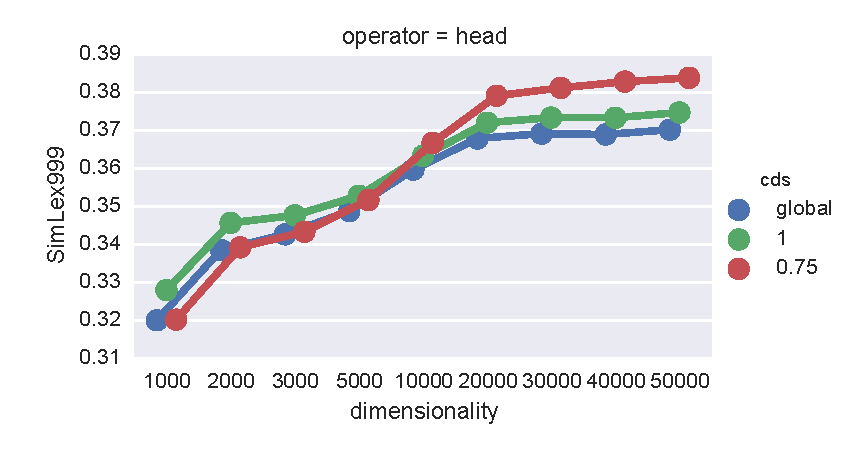
\includegraphics[width=0.5\textwidth]{supplement/figures/SimLex999-interaction-cds}
  \caption{SimLex-999 influence of \texttt{cds}.}
  \label{fig:SimLex999-cds}
\end{wrapfigure}


Models that do not perform shifting (abbreviated as N/A in Figure~\ref{fig:SimLex999-neg}), peak at 20\,000 dimensions and decrease afterwards with increasing variance. With 10\,000 dimensions or more they are statistically different from the best result.

There is no statistically significant difference between SPMI and SCPMI performance with a slight advantage to SCPMI (Figure~\ref{fig:SimLex999-discr}): PMI value compression into the range of $(0; 1)$ is unnecessary for lexical tasks (H\ref{hyp:lex-pmi-cpmi}).

Finally, models benefit from context distribution smoothing; spaces with less than 10\,000 dimensions produce the best results with $\alpha = 1$. For spaces with higher dimensionality, $\alpha = 0.75$ is the most advantageous (Figure~\ref{fig:SimLex999-cds}). However, the difference between $\alpha = 1$ and $\alpha = 0.75$ is statistically insignificant. H\ref{hyp:cds} (smoothing is beneficial for high-dimensional spaces) is not supported.

\subsection{Difference between Max selection and heuristics on SimLex-999}

As expected, manual, heuristic-based parameter selection is more homogeneous, as Table~\ref{tab:Simlex999-heuristics-selection} shows. Both selection models agree on parameters for high-dimensional spaces ($D \geq 2\,000$), with an exception of similarity: Max selection prefers cosine, while manual prefers correlation-based similarity measures. Because of this, manual selection does not pick the best result for the 2\,000 dimensional model, but at 50\,000 dimensions a model selected manually scores only 0.001 lower: 0.384 versus 0.385 as also seen on Figure~\ref{fig:SimLex999-results}.

The average relative difference between Max selection and heuristics is 0.039 (3.9\%), which is within the 10\% margin set by H\ref{hyp:10percent}. Moreover, statistically significant difference between the results is only for the models with dimensionality of 1\,000, 2\,000 and 3\,000.

\section{Experiments on MEN dataset}
\label{sec:men}

\begin{figure}
  \centering

    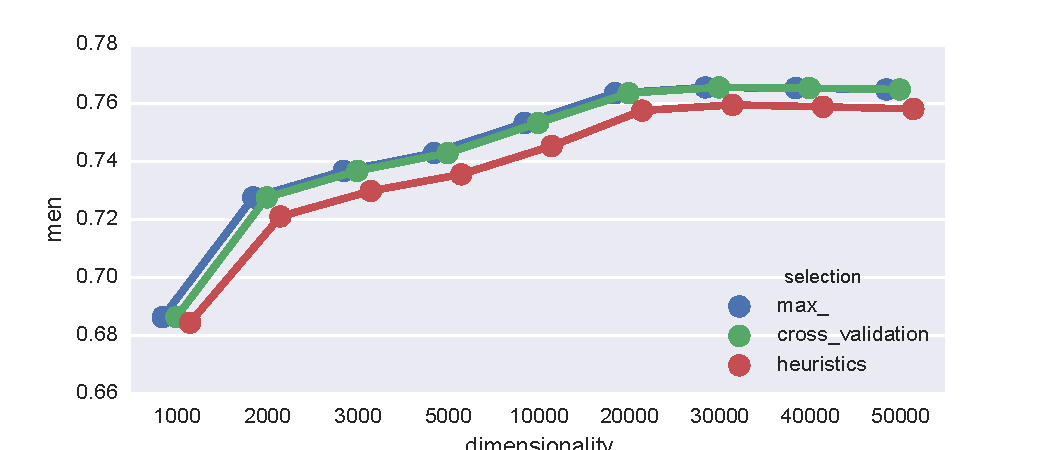
\includegraphics[width=0.5\textwidth]{supplement/figures/men-results}
  \caption{MEN results.}
  \label{fig:men-results}
\end{figure}

%%% Local Variables:
%%% mode: latex
%%% TeX-master: "../thesis"
%%% End:


The MEN test collection consists of 3\,000 word pairs judged for similarity \cite{Bruni:2014:MDS:2655713.2655714}. In contrast to SimLex-999, the dataset does not distinguish between similarity and relatedness. As with SimLex-999, the models are evaluated by the Spearman's-$\rho$ correlation. The minimum significant difference for MEN $\sigma^{0.9}_{0.05} = 0.013$.

\subsection{Max selection}
\label{sec:max-selection-men}

\begin{table}[b]
  \centering

  \begin{tabular}{rrlllrl}
\toprule
 dimensionality &    men &  freq &  discr &     cds &  neg &   similarity \\
\midrule
           1\,000 &  0.686 &     1 &  scpmi &  global &  1.4 &  correlation \\
           2\,000 &  0.728 &  logn &  scpmi &       1 &  0.7 &          cos \\
           3\,000 &  0.737 &  logn &  scpmi &       1 &  0.7 &          cos \\
           5\,000 &  0.743 &  logn &  scpmi &    0.75 &  0.7 &          cos \\
          10\,000 &  0.753 &  logn &  scpmi &    0.75 &  1.0 &  correlation \\
          20\,000 &  0.763 &  logn &  scpmi &    0.75 &  1.0 &  correlation \\
          \textbf{30\,000} &  \textbf{0.765} &  \textbf{logn} &  \textbf{scpmi} &    \textbf{0.75} &  \textbf{1.0} &  \textbf{correlation} \\
          \textbf{40\,000} &  \textbf{0.765} &  \textbf{logn} &  \textbf{scpmi} &    \textbf{0.75} &  \textbf{1.0} &  \textbf{correlation} \\
          \textbf{50\,000} &  \textbf{0.765} &  \textbf{logn} &  \textbf{scpmi} &    \textbf{0.75} &  \textbf{1.0} &  \textbf{correlation} \\
\bottomrule
\end{tabular}


  \caption{MEN Max selection}
  \label{tab:men-max-selection}
\end{table}


Figure~\ref{fig:men-results} shows the selection results. Again, cross-validation results are identical with Max selection. Table~\ref{tab:men-max-selection} shows the results together with the selected models.

Model performance monotonically increases as dimensionality increases. The highest score of 0.765 is achieved by 3 spaces with $D \geq 30\,000$, \logNSCPMI/, smoothed context distribution ($\alpha = 0.75$), shifted PMI values ($k = 1$) and the similarity measure based on correlation. Models with the same parameter choice, but lower dimensionality (10\,000 and 20\,000) are statistically indistinguishable from the highest scoring models.

In comparison with SimLex-999, models with ``more extreme'' parameters give better results on MEN. For example, $\alpha = 0.75$ is the best for models tested on SimLex-999 with dimensionality starting with 20\,000, while for models tested on MEN, this parameter choice is the best starting with 5\,000. Similar behaviour is observed for \texttt{neg} and similarity. For high-dimensional spaces, the switch from SimLex-999 to MEN changes the best \texttt{neg} choice from 0.7 to 1 and similarity from cosine to correlation. Such a difference in parameter choices might suggest the difference between \textit{relatedness} and \textit{similarity}, but it still supports H\ref{hyp:freq}, H\ref{hyp:cds} and H\ref{hyp:neg} that frequency, context distribution smoothing and sparsity are important for high-dimensional spaces. H\ref{hyp:similarity} is also supported, as correlation is the best similarity measure for high-dimensional spaces.

\subsection{Heuristics}
\label{sec:heuristics-men}

\begin{table}
  \centering

  \begin{tabular}{rrlllll}
\toprule
 dimensionality &    men &  freq & discr &     cds & neg &   similarity \\
\midrule
           1\,000 &  0.684 &  logn &  spmi &  global &   2 &  correlation \\
           2\,000 &  0.721 &  logn &  spmi &  global &   2 &  correlation \\
           3\,000 &  0.730 &  logn &  spmi &  global &   2 &  correlation \\
           5\,000 &  0.735 &  logn &  spmi &  global &   2 &  correlation \\
          10\,000 &  0.745 &  logn &  spmi &  global &   2 &  correlation \\
          20\,000 &  0.757 &  logn &  spmi &  global &   5 &  correlation \\
          \textbf{30\,000} &  \textbf{0.759} &  \textbf{logn} &  \textbf{spmi} &  \textbf{global} &   \textbf{5} &  \textbf{correlation} \\
          \textbf{40\,000} &  \textbf{0.759} &  \textbf{logn} &  \textbf{spmi} &  \textbf{global} &   \textbf{5} &  \textbf{correlation} \\
          50\,000 &  0.758 &  logn &  spmi &  global &   5 &  correlation \\
\bottomrule
\end{tabular}


  \caption{MEN selection based on heuristics. The highest value is 0.759. The
    values that are greater than 0.746 are indistinguishable from the highest score.}
  \label{tab:men-heuristics-selection}
\end{table}


\begin{wraptable}[11]{O}{0.5\textwidth}
  \vspace{1em}
  \centering

  \begin{tabular}{lr}
\toprule
      parameter &  partial $R^2$ \\
\midrule
            neg &  0.309 \\
           freq &  0.204 \\
     similarity &  0.183 \\
          discr &  0.119 \\
 dimensionality &  0.108 \\
            cds &  0.086 \\
\bottomrule
\end{tabular}


  \caption{MEN feature ablation}
  \label{tab:men-ablation}
\end{wraptable}

The linear model gives an adjusted $R^2$ of 0.733, which is lower than on SimLex-999, but is still high. Table~\ref{tab:men-ablation} shows partial $R^2$ scores for the explored parameters. The most influential parameter is \texttt{neg}, followed by \texttt{freq} and similarity. This is different from the case of SimLex-999, where the parameter's influence ``order'' is reversed.

\begin{figure}
% \begin{wrapfigure}{O}{0.5\textwidth}
  % \vspace{-30pt}
  \centering

  \begin{subfigure}[t]{0.49\textwidth}
    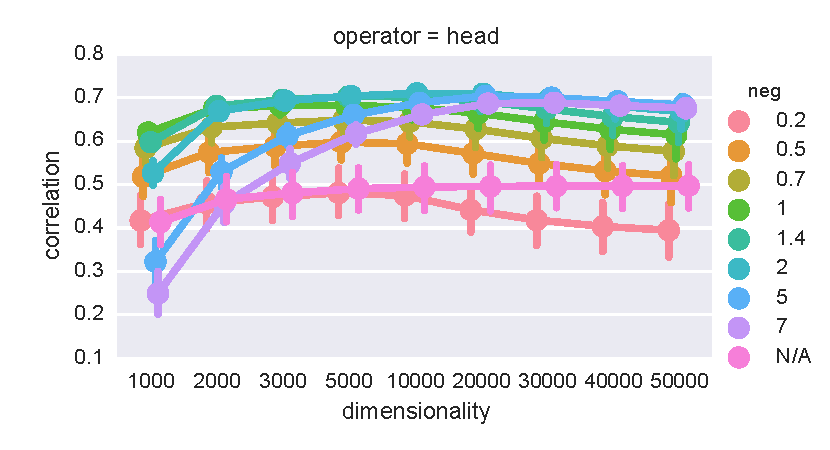
\includegraphics[width=\textwidth]{supplement/figures/men-interaction-neg}

  \caption{\texttt{neg}}
  \label{fig:men-neg}
  \end{subfigure}
  \begin{subfigure}[t]{0.49\textwidth}
    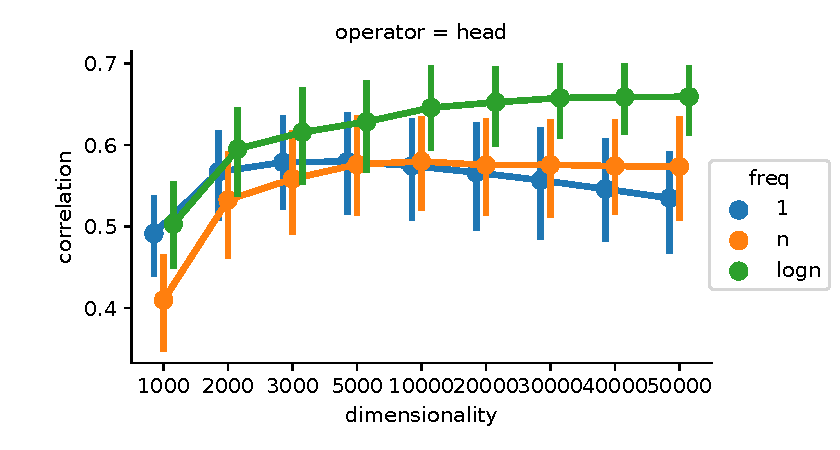
\includegraphics[width=\textwidth]{supplement/figures/men-interaction-freq}

  \caption{\texttt{freq}}
  \label{fig:men-freq}
  \end{subfigure}

  \caption{MEN.}
\end{figure}
 The parameter \texttt{neg}, which controls sparsity, with $k = 2$ is preferable for spaces with dimensionality less than 20\,000. For spaces with more dimensions, $k = 5$ is more beneficial (Figure~\ref{fig:men-neg}). Models without shifting and with $k$ set to 0.2, 0.5, 0.7 and 7 are statistically significantly different from the best choice for all dimensions. This replicates the suggestions of \newcite{TACL570}. We, however, expect that for spaces with more than 50\,000 dimensions even higher values should be preferred.

The choice of $k = 1$ with $D \ge 3\,000$ is statistically indistinguishable from the best choice, $k = 1.4$ is statistically indistinguishable with $D \ge 20\,000$, $k = 2$ is statistically indistinguishable for $2\,000 \le D \le 40\,000$ and $k = 5$ is statistically indistinguishable when $D \le 10\,000$.

The choice of $k$ for MEN contrasts with the heuristics derived from SimLex-999, where the \texttt{neg} values of 0.5, 0.7 and 1 are statistically indistinguishable from each other, but still complies with H\ref{hyp:neg}: sparse high-dimensional spaces outperform their high-dimensional, but dense counterparts. The performance of the models with less than 20\,000 dimensions is statistically different.

Regarding the frequency component, $\log n$ outperforms all other choices (Figure~\ref{fig:men-freq}). With 2\,000 or more dimensions it is statistically significantly different from the constant frequency. It is always statistically significantly different from the linear frequency. H\ref{hyp:freq}---that frequency is needed for high-dimensional spaces---is once again confirmed.

\begin{figure}[b]
% \begin{wrapfigure}{O}{0.5\textwidth}
  % \vspace{-30pt}
  \centering
  \begin{subfigure}[t]{0.49\textwidth}
    \hspace{-20pt}
    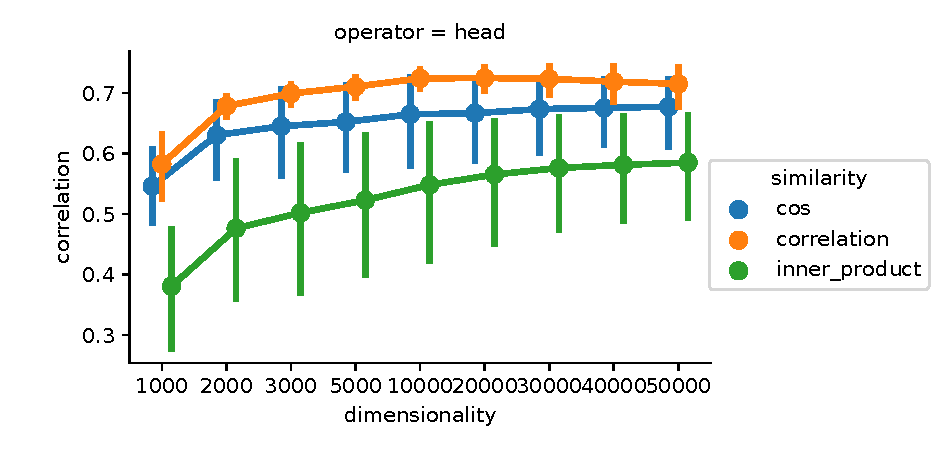
\includegraphics[width=1.1\textwidth]{supplement/figures/men-interaction-similarity}

  \caption{MEN influence of similarity.}
  \label{fig:men-similarity}
  \end{subfigure}
  \begin{subfigure}[t]{0.49\textwidth}
    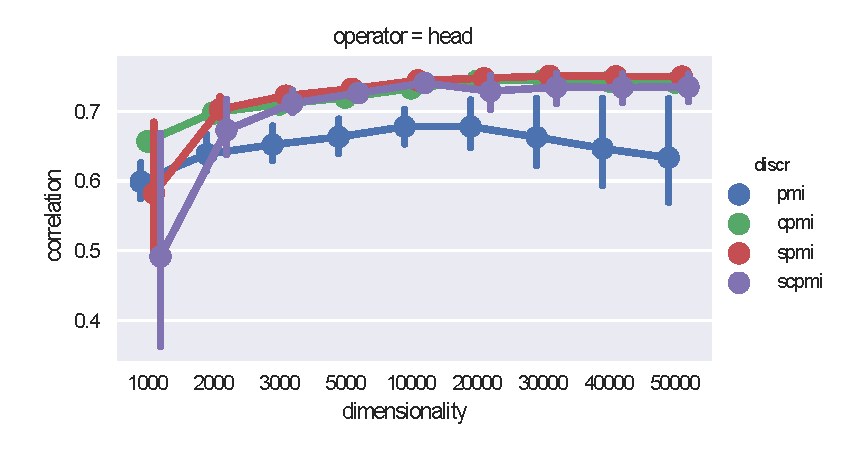
\includegraphics[width=\textwidth]{supplement/figures/men-interaction-discr}

  \caption{MEN influence of \texttt{discr}.}
  \label{fig:men-discr}
  \end{subfigure}
\end{figure}


Correlation is the preferred similarity measure (Figure~\ref{fig:men-similarity}) it is statistically significantly different from both cosine and the inner product. This is, again, in line with the choice based on SimLex-999. However, the gap between cosine and correlation similarities stays constant, with an exception of $D = 1\,000$, where the gap is smaller, giving a weak support to H\ref{hyp:similarity}: correlation performs best with high-dimensional spaces.

\begin{figure}
%\begin{wrapfigure}[9]{O}{0.5\textwidth}
  % \vspace{-30pt}
  \centering

  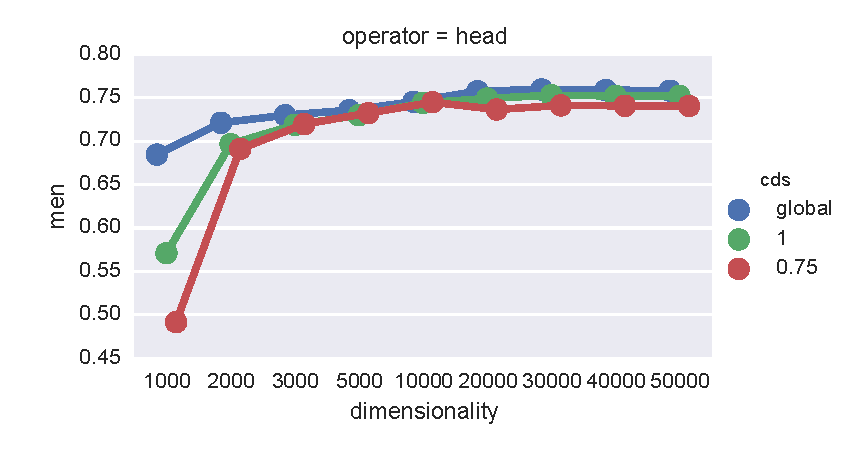
\includegraphics[width=0.5\textwidth]{supplement/figures/men-interaction-cds}

  \caption{MEN influence of \texttt{cds}}
  \label{fig:men-cds}
\end{figure}


Overall, SPMI is the preferred discriminativeness (Figure~\ref{fig:men-discr}), however, it is closely followed by CPMI (the statistically significance difference for $D \le 2\,000$) and SCPMI (is statistically indistinguishable for $3\,000 \le D \le 10\,000$). This contrasts with SimLex-999, where SCPMI is preferred. However, in both cases, the difference between the two choices is minimal. This is consistent with H\ref{hyp:lex-pmi-cpmi} that lexical models do not need PMI compression.

Global context probability gives on average higher results for MEN (Figure~\ref{fig:men-cds}). For models with 3\,000 or more dimensions, local probabilities are statistically indistinguishable. For models with $2\,000< D < 20,000$, $\alpha = 0.75$ is statistically indistinguishable as well.

Note that SimLex-999 prefers context distribution smoothing (Figure~\ref{fig:SimLex999-cds}). The difference in performance between local context probabilities and global context probabilities decreases as dimensionality increases, making a weak support of H\ref{hyp:cds} that high-dimensional spaces benefit from context distribution smoothing.

\subsection{Difference between Max selection and heuristics on MEN}

The two selection procedures agree on fewer parameters than the ones based on SimLex-999. Both agree on discrimination ($\log n$) and similarity score for spaces with dimensionality greater than 10\,000 (correlation).

While SCPMI is chosen by Max selection, SPMI is preferred by the selection based on heuristics, however, the difference between the two is minimal, especially for $3\,000 \le D \le 10\,000$, where the difference is statistically in significant.

In contrast to the Max selection, which chooses the models with context distribution smoothing, heuristics prefers models with global context probabilities. However, with $3\,000 < D <20\,000$, there is no statistically significant difference between \texttt{cds} values.

Also, heuristics picks models with higher shifting values $k$ (2 and 5), in contrast to Max selection, where 0.7 and 1 are chosen. Table~\ref{tab:men-heuristics-selection} summarises the parameter selection based on heuristics.

The average relative difference between Max selection and heuristics is 0.008 (0.8\%), supporting H\ref{hyp:10percent}: the difference between Max selection and heuristics is within the 10\% margin. Moreover, the difference in scores between the two selections is statistically insignificant.

\subsection{Difference between heuristics based on MEN and SimLex-999}

Heuristics based on MEN agree with ones based on SimLex-999 for two parameters: frequency ($\log n$) and similarity (correlation). The methods disagree on \texttt{discr} (SCPMI versus SPMI, respectively). However, the difference is negligible, because the compression of PMI values should not affect lexical similarity, as we expect by H\ref{hyp:lex-pmi-cpmi}. Context distribution (smoothed versus global) and shifting parameter (higher values of $k$ perform better on MEN) are other differences between the parameter selection based on the two datasets.

\section{Transfer of selected models between datasets}
\label{sec:select-model-transf}

We have identified parameters that lead to high correlation scores with human similarity judgements. However, we did not check whether the chosen models overfit. By transferring chosen models across datasets, that is taking parameters that are good on one dataset and applying them on another dataset, we should see whether chosen models overfit. 

\subsection{From SimLex-999 to MEN}
\label{sec:simlex-men}

\begin{figure}
  \centering

  \begin{subfigure}[t]{0.49\textwidth}
    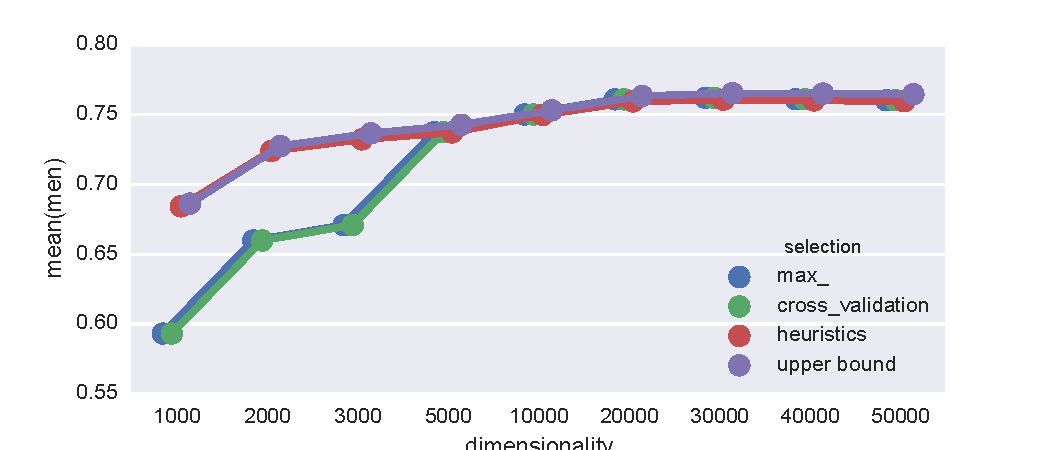
\includegraphics[width=\textwidth]{supplement/figures/SimLex999-transfer}
    \caption{Transfer from SimLex-999 to MEN}
    \label{fig:SimLex999-transfer}
  \end{subfigure}
  \begin{subfigure}[t]{0.49\textwidth}
    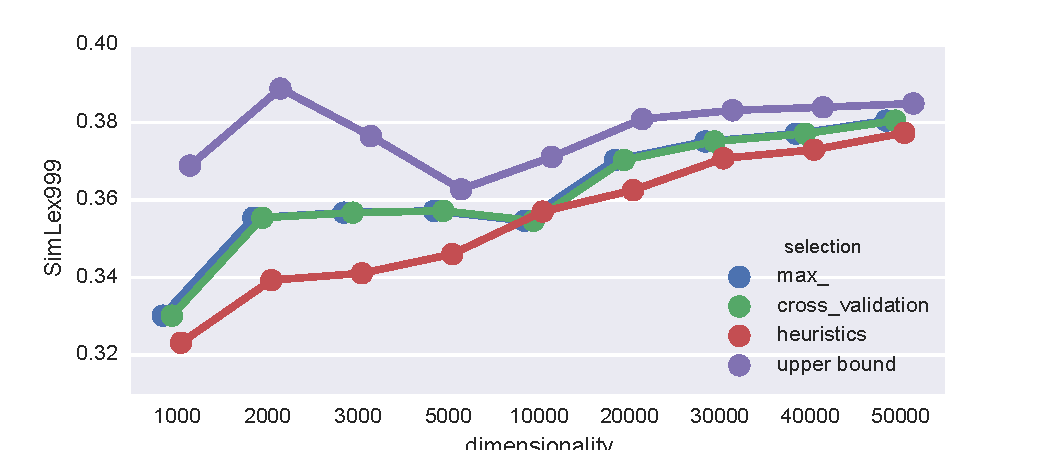
\includegraphics[width=\textwidth]{supplement/figures/men-transfer}
    \caption{Transfer from MEN to SimLex-999}
    \label{fig:men-transfer}
  \end{subfigure}

  \caption{Model transfer between lexical evaluation datasets}
  \label{fig:lexical-transfer}
\end{figure}

%%% Local Variables:
%%% mode: latex
%%% TeX-master: "../thesis"
%%% End:


The models selected using heuristics based on the SimLex-999 dataset perform well on MEN: for all dimensions, the selected models are statistically indistinguishable from the best possible score (Figure~\ref{fig:SimLex999-transfer}). The average relative difference with the upper bound is 0.006, or 0.6\%.

The Max-based selection is statistically indistinguishable the upper bound for models with dimensionality greater than 5\,000. The average relative difference with the upper bound is 0.039. The higher difference is due to overfitting of the low-dimensional models ($D < 5\,000$), where the average relative difference is 0.09.

In this case, heuristic-based selection leads to better performance than the Max-based selection, supporting H\ref{hyp:overfitting}: Max selection does overfit.

\subsection{From MEN to SimLex-999}

Heuristics transferred from MEN to SimLex-999 behave less efficiently, they do not always outperform Max selection, though for high-dimensional spaces (5\,0000 dimensions and more) the difference is statistically insignificant (Figure~\ref{fig:men-transfer}). The average relative difference is 0.062, which is ten times more than the transition from SimLex-999 to MEN.

Neither Max selection picks the best possible results when transferred from MEN to SimLex-999, the difference with the best scores is statistically insignificant with 3\,000 and more dimensions.The average relative difference is lower than with heuristics: 0.042 versus 0.062. This is similar to the transition in other direction.

Max-based selection leads to better performance than the heuristics for MEN, making a case against H\ref{hyp:overfitting}: Max selection does not overfit.

\section{Universal parameter selection for lexical datasets}
\label{sec:universal-lexical-param-selection}

This section explores whether there are models that behave well across several datasets. It serves two interests. First of all, both datasets measure similarity, so the underlying method of estimating it ideally should not depend on the dataset. Secondly, by compromising between the two datasets, overfitting should be avoided.

We score the models based on the average of the normalised scores over SimLex-999 and MEN:
\begin{equation}
\label{eq:score-lexical}
\operatorname{score}_\mathit{lexical}(\mathit{model}) =%
\frac{1}{2}\times%
\frac{\operatorname{score}_\mathit{SimLex-999}(\mathit{model})}%
{\max_m\operatorname{score}_\mathit{SimLex-999}(m)}%
+%
\frac{1}{2}\times%
\frac{\operatorname{score}_\mathit{MEN}(\mathit{model})}%
{\max_m\operatorname{score}_\mathit{MEN}(m)}%
\end{equation}

This is the simplest scoring methods. It treats the datasets equally by giving equal weights to them, without giving any preferences. We normalise the scores to compensate for various magnitudes of representative results between SimLex-999 and MEN.

The performance of the selected models on both datasets and the normalised average is shown in Table~\ref{tab:lexical-max-selection} (Max selection) and Table~\ref{tab:lexical-heuristics-selection} (selection based on heuristics) and in Figure~\ref{fig:lexical-results}.

\begin{table}
  \centering

  \begin{tabular}{rrrrlllrl}
\toprule
 dimensionality &  SimLex999 &    men &  lexical &  freq &  discr &     cds &  neg & similarity \\
\midrule
           1\,000 &      0.347 &  0.682 &    0.892 &     1 &   spmi &  global &  1.4 &        cos \\
           2\,000 &      0.361 &  0.722 &    0.936 &  logn &  scpmi &  global &  1.0 &        cos \\
           3\,000 &      0.357 &  0.737 &    0.940 &  logn &  scpmi &       1 &  0.7 &        cos \\
           5\,000 &      \textbf{0.363} &  0.742 &    0.951 &  logn &  scpmi &       1 &  0.7 &        cos \\
          10\,000 &      \textbf{0.371} &  \textbf{0.750} &    0.967 &  logn &  scpmi &       1 &  0.7 &        cos \\
          20\,000 &      \textbf{0.381} &  \textbf{0.761} &    0.987 &  logn &  scpmi &    0.75 &  0.7 &        cos \\
          30\,000 &      \textbf{0.383} &  \textbe{0.762} &    0.991 &  logn &  scpmi &    0.75 &  0.7 &        cos \\
          40\,000 &      \textbf{0.384}  &  \textbf{0.761} &    0.991 &  logn &  scpmi &    0.75 &  0.7 &        cos \\
          50\,000 &     \textbe{ 0.385} &  \textbf{0.760} &    \textbe{0.992} &  logn &  scpmi &    0.75 &  0.7 &        cos \\
\bottomrule
\end{tabular}


  \caption[Lexical (combined SimLex-999 and MEN) Max selection]{Lexical (combined SimLex-999 and MEN) Max selection. For the
    individual dataset scores, the scores in bold are indistinguishable from the
  highest score. For SimLex-999, the highest score is 0.385 and the scores above
0.362 are indistinguishable. For MEN, the highest score is 0.762 and the scores
above 0.749 are indistinguishable. The highest combined score is 0.992 and the scores above 0.954 are indistinguishable.}
  \label{tab:lexical-max-selection}
\end{table}


To calculate the minimal required difference for statistical significance
(MRDS), the MRDS of the corresponding datasets are put in to formula
(\ref{eq:score-lexical}). The resulting MRDS value is $\sigma^{0.9}_{0.05} = 0.038$.

\subsection{Max selection}
\label{sec:max-selection}

In general, the more dimensions, the better the results are. The selection yields the best results at $D = 50\,000$ for SimLex-999 and at $D = 30\,000$ for MEN. While for SimLex-999, the Max selection is statistically indistinguishable from the best score with 5\,000 and more dimensions. For MEN, the performance peaks at 30\,000 dimensions and then slightly deviates from the upper bound as the dimensionality increases, however, it is statistically indistinguishable from the highest score with 10\,000 and more dimensions.

The Max selection based on the combination of the two lexical datasets is closer to the Max selection based on SimLex-999 (Table~\ref{tab:Simlex999-max-selection}) than on MEN (Table~\ref{tab:men-max-selection}).

\begin{figure}[b]
  \centering

  \begin{subfigure}[t]{0.49\textwidth}
    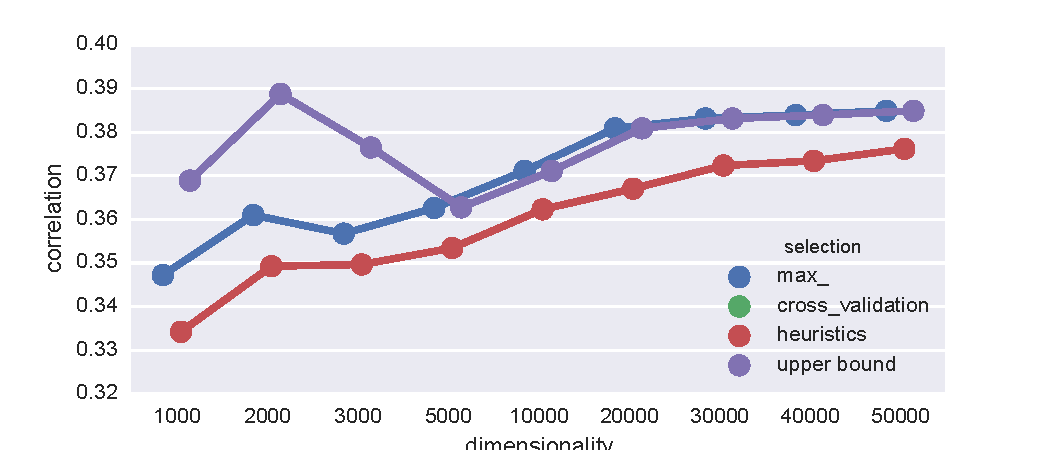
\includegraphics[width=\textwidth]{supplement/figures/lexical-results-SimLex999}
    \caption{SimLex-999}
    \label{fig:lexical-results-simlex}
  \end{subfigure}
  \begin{subfigure}[t]{0.49\textwidth}
    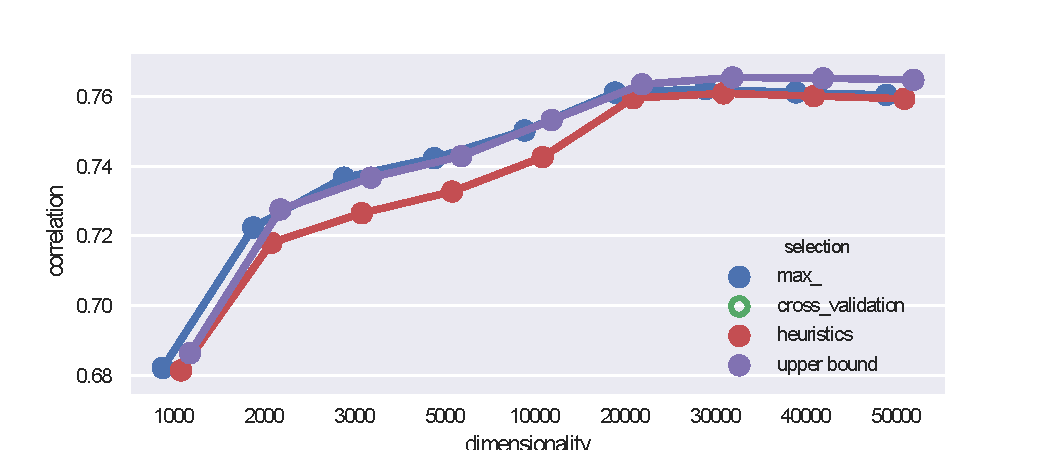
\includegraphics[width=\textwidth]{supplement/figures/lexical-results-men}
    \caption{MEN}
    \label{fig:lexical-results-men}
  \end{subfigure}

  \caption{Performance of models based on the selection over the average lexical performance}
  \label{fig:lexical-results}
\end{figure}

%%% Local Variables:
%%% mode: latex
%%% TeX-master: "../thesis"
%%% End:


\subsection{Heuristics}

\begin{table}
  \centering

  \begin{tabular}{rrrrlllll}
\toprule
 dimensionality &  SimLex999 &   men &  lexical &  freq &  discr &     cds & neg &   similarity \\
\midrule
           1\,000 &       0.33 &  0.68 &     0.87 &  logn &  scpmi &  global &   1 &  correlation \\
           2\,000 &       0.35 &  0.72 &     0.92 &  logn &  scpmi &  global &   1 &  correlation \\
           3\,000 &       0.35 &  0.73 &     0.92 &  logn &  scpmi &  global &   1 &  correlation \\
           5\,000 &       0.35 &  0.73 &     0.93 &  logn &  scpmi &  global &   1 &  correlation \\
          10\,000 &       0.36 &  0.74 &     0.95 &  logn &  scpmi &  global &   1 &  correlation \\
          20\,000 &       0.37 &  \textbf{0.76} &     0.97 &  logn &  scpmi &  global &   2 &  correlation \\
          30\,000 &       0.37 &  \textbf{0.76} &     \textbf{0.98} &  logn &  scpmi &  global &   2 &  correlation \\
          40\,000 &       0.37 &  \textbf{0.76} &     \textbf{0.98} &  logn &  scpmi &  global &   2 &  correlation \\
          50\,000 &       \textbf{0.38} &  \textbf{0.76} &     \textbf{0.98} &  logn &  scpmi &  global &   2 &  correlation \\
\bottomrule
\end{tabular}


  \caption{Lexical (combined SimLex-999 and MEN) selection based on heuristics.}
  \label{tab:lexical-heuristics-selection}
\end{table}


The linear model achieves an adjusted $R^2$ of 0.817, which is less than the $R^2 = 0.867$ of SimLex-999, but is greater than the $R^2 = 0.733$ of MEN. Table~\ref{tab:lexical-ablation} shows partial $R^2$s for each parameter---the most influential are similarity, \texttt{neg} and \texttt{freq}.

\begin{figure}[b]
% \begin{wrapfigure}{O}{0.5\textwidth}
  % \vspace{-30pt}
  \centering

  \begin{subfigure}[t]{0.49\textwidth}
    \hspace{-20pt}
    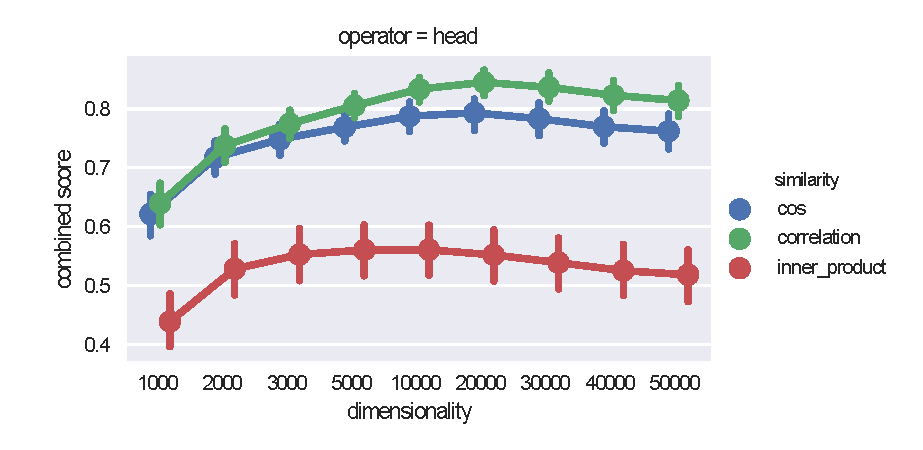
\includegraphics[width=1.1\textwidth]{supplement/figures/lexical-interaction-similarity}

    \caption{Similarity}
    \label{fig:lexical-similarity}
  \end{subfigure}
  \begin{subfigure}[t]{0.49\textwidth}
    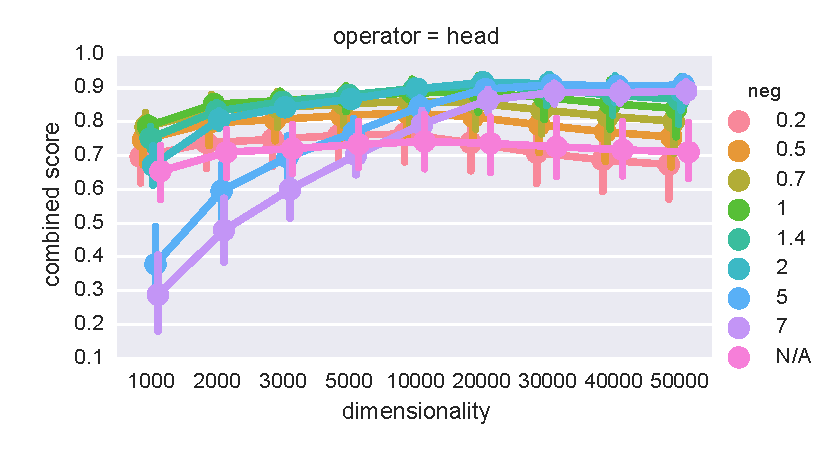
\includegraphics[width=\textwidth]{supplement/figures/lexical-interaction-neg}

    \caption{\texttt{neg}}
    \label{fig:lexical-neg}
  \end{subfigure}
  \caption{Lexical the influence of similarity and \texttt{neg}}
\end{figure}
 Correlation is the similarity measure of choice (Figure~\ref{fig:lexical-similarity}). However, the difference between cosine and correlation is not statistically significant for $D < 10\,000$ supporting H\ref{hyp:similarity} that correlation is beneficial for high-dimensional spaces.

\begin{wraptable}[13]{O}{0.5\textwidth}
  \vspace{3em}
  \centering

  \begin{tabular}{lr}
\toprule
      parameter &  partial $R^2$ \\
\midrule
     similarity &    0.299 \\
            neg &    0.280 \\
           freq &    0.231 \\
 dimensionality &    0.095 \\
          discr &    0.095 \\
            cds &    0.076 \\
\bottomrule
\end{tabular}


  \caption{Lexical feature ablation}
  \label{tab:lexical-ablation}
\end{wraptable}


For the models with dimensionality less than 20\,000, shifting should be used with $k = 1$, otherwise, $k = 2$ is preferred (Figure~\ref{fig:lexical-neg}). This supports H\ref{hyp:neg} that the more dimensions a model has the sparser it should be.

The choices of $k$ set to 0.2, 0.5 and N/A lead to the scores that are statistically significantly different from the best score. Shifting $k = 0.7$ leads to the statistically different results with $D \ge 20,000$; $k = 1$ with $D \ge 30\,000$; $k = 1.4$ with $D = 50\,000$; $k = 2$ with $D \le 2\,000$; $k = 5$ with $D \le 10\,00$; and $k = 7$ with $D \le 20$.

\begin{figure}[h]
% \begin{wrapfigure}{O}{0.5\textwidth}
  % \vspace{-30pt}
  \centering

  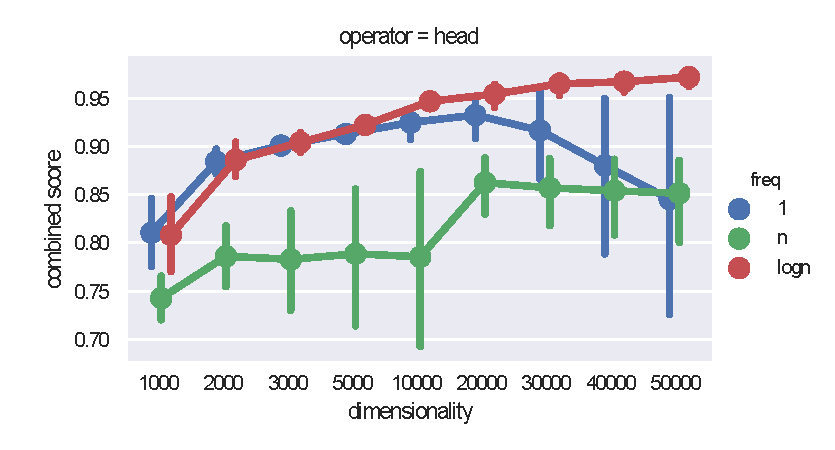
\includegraphics[width=0.5\textwidth]{supplement/figures/lexical-interaction-freq}

  \caption{Lexical influence of \texttt{freq}.}
  \label{fig:lexical-freq}
\end{figure}
 The frequency parameter $\log n$, on average, performs the best as the frequency component (Figure~\ref{fig:lexical-freq}). But for $D < 30\,000$, 1 performs statistically indistinguishably, supporting H\ref{hyp:freq} that the frequency component is most useful for high-dimensional spaces.

SCPMI is the preferred discrimination component, but SPMI is statistically
insignificantly different to it (Figure~\ref{fig:lexical-discr}), backing up H\ref{hyp:lex-pmi-cpmi} that PMI value compression is not needed in lexical tasks.

% \begin{figure}[h]
\begin{wrapfigure}[7]{O}{0.5\textwidth}
  \vspace{-30pt}
  \centering

  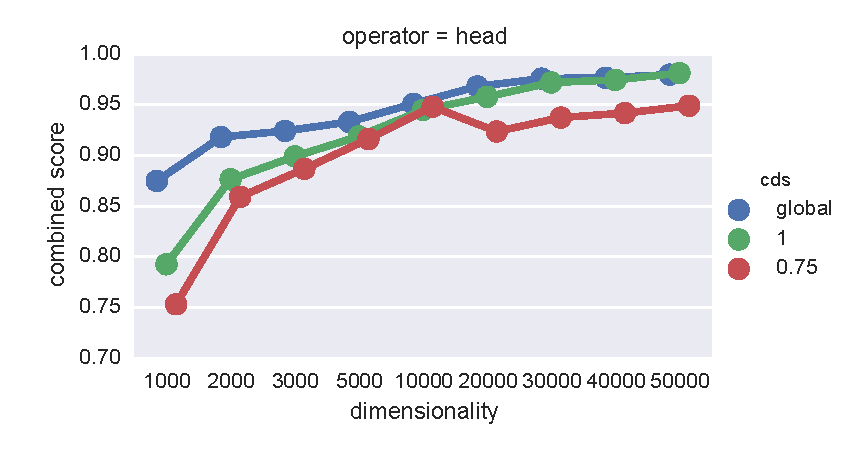
\includegraphics[width=0.5\textwidth]{supplement/figures/lexical-interaction-cds}

  \caption{Lexical influence of \texttt{cds}.}
  \label{fig:lexical-cds}
\end{wrapfigure}
 Global context probabilities, on average, behave the best (Figure~\ref{fig:lexical-cds}). However, global context probabilities and local context probabilities with $\alpha = 1$ yield statistically insignificantly different results for $D > 2\,000$, giving support to H\ref{hyp:cds} that context distribution smoothing is needed in high-dimensional spaces.

\subsection{Comparison with single dataset based selections}

Both selection methods mostly agree on frequency ($\log n$) and discriminativeness (SCPMI).

Context probability distribution smoothing varies between the selection methods but follows the corresponding procedures based on MEN.

The Max-based selection for \texttt{neg} follows the Max selection on SimLex-999.

Even though the similarity choice is different between the Max-based and heuristic-based selections, it is consistent with SimLex-999 in both cases and with MEN for the heuristic-based selection.

For the Max-based selection, the average difference is 0.020 on SimLex-999 and 0.004 for MEN.

For the heuristics-based selection, the average difference is 0.048 for SimLex-999 and 0.010 for MEN, which is within the 10\% limit set by H\ref{hyp:10percent}.

Max selection behaves better than the heuristics-based selection on the average difference, but we cannot check how well these two selections behave on other lexical datasets. This is evidence against H\ref{hyp:overfitting} suggesting that testing on multiple datasets avoids overfitting and manual selection becomes too conservative.

Based on the experiments, \logNSCPMI/ with shifting close to 1 is the quantification of choice for the lexical tasks, however, more work needs to be done to find a robust choice for context distribution smoothing and similarity measure.

\section{Conclusion}
\label{sec:conclusion-lexical}

Lexical experiments give support to most of the stated hypotheses. The optimal parameter choice depends on dimensionality (H\ref{hyp:dimen}). In particular, non constant frequency component (H\ref{hyp:freq}), context distribution smoothing (H\ref{hyp:cds}) and shifting (H\ref{hyp:neg}) are recommended to be applied for spaces with $D \geq 10\,000$.

The switch at 10\,000 dimensions is a ``parameter sweet spot,'' as parameter choice is not significant at these points; the most representative example of this is the behaviour of \texttt{cds} on SimLex-999 (Figure~\ref{fig:SimLex999-cds}). After that point, performance either converges (supporting H\ref{hyp:var}), as in the case of \texttt{neg} on SimLex-999 (Figure~\ref{fig:SimLex999-neg}), or there is one dominant choice, as for \texttt{freq} on SimLex-999 (Figure~\ref{fig:SimLex999-freq}).

As expected, we did not see a significant influence of the ``compression'' of the PMI values (H\ref{hyp:lex-pmi-cpmi}).

We could not find supporting evidence for H\ref{hyp:overfitting}, as Max-selected models performed well on transfer and do not overfit. Both selection methods are within the 10\% difference margin to the highest result (H\ref{hyp:10percent}), suggesting that there indeed might be a universal vector space (H\ref{hyp:universal}).

%\begin{wraptable}[12]{O}{0.5\textwidth}
\begin{table}
\centering
  \begin{tabular}{lll}
    \toprule
    Model           & SimLex-999 & MEN \\
    \midrule
    PPMI$^*$        &         0.393      & 0.745 \\
    SVD$^*$         & \textbf{0.432}     & \textbe{0.778} \\
    SGNS$^*$        & \textbe{0.438}     & \textbf{0.774} \\
    GloVe$^*$       &         0.398      & 0.729 \\
    \addlinespace
    This work       &         0.384      & 0.764 \\
    \bottomrule
  \end{tabular}
  \caption[Comparison with other lexical models]{Our models in comparison to the previous work on lexical tasks. $^*$Results reported by \newcite{TACL570}.}
\label{tab:lexical-comparison}
\end{table}
 On lexical tasks, the best results among the selected models are 0.384 (SimLex-999) and 0.764 (MEN). On the similarity dataset, scores are 0.009 points below the PPMI model of \newcite{TACL570}, the difference is not statistically significant. On the relatedness dataset, our score is 0.019 points above \citet{TACL570}, the difference is statistically significant. Note the difference in dimensionality (50\,000 in this work, 189\,533 in the other work), source corpora (2.8 billion tokens from  ukWaC and WaCkypedia in this work, 1.5 billion tokens from an August 2013 Wikipedia dump) and window size (5 versus 2). Table~\ref{tab:lexical-comparison} shows the results of SVD, SGNS and GloVe-based vector spaces are given for comparison.

The next step is to test compositional models. Before experiments are presented in Chapter~\ref{sec:sentential}, a new dataset that provides relevance judgements of pairs of sentences is presented in Chapter~\ref{sec:phraserel}.

%%% Local Variables:
%%% mode: latex
%%% TeX-master: "thesis"
%%% TeX-engine: xetex
%%% End:
